%% !TEX program = xelatex
\documentclass[12pt,final]{novelette} % font size, twoside, twocolumn, draft-final, use extarticle for 8-20pt

\title{Calculus III Midterm 2568}
\author{Kaka Cring}
\date{\today}

% !TEX root = calculus_iii_midterm.tex
\settasks{
    label=\arabic*.,
    label-align=left,
    label-width=0.8em
}

\setlength\headheight{0pt}  % header height
\setlength\footskip{48pt}    % space before base of footer
\addtolength\textheight{40pt}
\renewcommand{\headrulewidth}{0pt} % width of header line
\fancyhead[L,R]{}
\fancyfoot[C]{\fbox{\bf หน้าที่ \thepage}}

\renewcommand{\qmark}[1]{\textit{(#1\ คะแนน)}}
\newcommand{\ansbox}{\ensuremath{\boxed{\hspace*{7em}\vphantom{\dfrac12}}} {}}
\newcommand{\ansboxs}{\ensuremath{\boxed{\hspace*{4em}\vphantom{\frac12}}} {}}
\newcommand{\ansboxl}{\ensuremath{\boxed{\hspace*{10em}\vphantom{\frac12}}} {}}
\newcommand{\ansboxL}{\ensuremath{\boxed{\hspace*{12em}\vphantom{\frac12}}} {}}
\newcommand{\ansboxq}{\ensuremath{\boxed{\hspace*{2em}\vphantom{\frac12}}} {}}
\newcommand{\ansboxi}[1]{\ensuremath{\boxed{\hspace*{#1}\vphantom{\frac12}}} {}}
\newcommand{\polarcoordinatecircle}{
    \medskip
    \begin{center}
        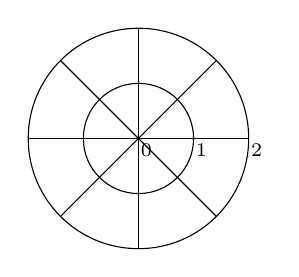
\begin{tikzpicture}[font=\scriptsize,scale=0.7]
            \draw (0,0) circle(1);
            \draw (0,0) circle(2);
            \foreach \i in {0,45,...,315} {
                    \draw (0,0) -- (\i:2);
                }
            \foreach \i in {0,1,2} {
                    \node[below,shift={(0.1,0.05)}] at (\i,0) {$\i$};
                }
        \end{tikzpicture}
        \hspace*{1cm}
    \end{center}
}
\usetikzlibrary{patterns}
\newcommand{\polarcoordinatetheta}{
    \begin{center}
        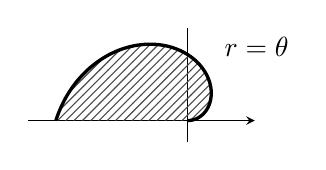
\begin{tikzpicture}
            \begin{axis}[
                    scale=0.42,
                    axis lines=middle,
                    y axis line style={-},
                    xmin=-3.8, xmax=1.6,
                    ymin=-0.5, ymax=2.2,
                    ticks=none,
                    axis equal image
                ]
                \addplot[
                    domain=0:pi,
                    samples=100,
                    pattern=north east lines,  % Hatching pattern
                    pattern color=black!70,
                    draw=none
                ]
                (
                {x*cos(deg(x))},
                {x*sin(deg(x))}
                )
                \closedcycle;
                \addplot[
                    domain=0:pi,
                    samples=100,
                    very thick,
                    black
                ]
                (
                {x*cos(deg(x))},
                {x*sin(deg(x))}
                );
            \end{axis}
            \node at (2.9, 1.2) {$r = \theta$};
        \end{tikzpicture}
        \hspace*{2.7cm}
    \end{center}
}
\newcommand{\polarcoordinatesintwotheta}{
    \begin{center}
        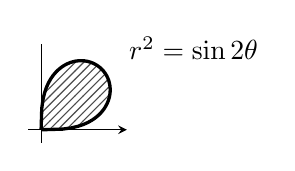
\begin{tikzpicture}
            \begin{axis}[
                    scale=0.22,
                    axis lines=middle,
                    y axis line style={-},
                    x=1cm, y=1cm,
                    xmin=-0.15, xmax=1,
                    ymin=-0.15, ymax=1,
                    ticks=none,
                    axis equal image
                ]
                \addplot[
                    domain=0:pi,
                    samples=100,
                    pattern=north east lines,  % Hatching pattern
                    pattern color=black!70,
                    draw=none
                ]
                (
                {sqrt(sin(deg(2*x))) * cos(deg(x))},
                {sqrt(sin(deg(2*x))) * sin(deg(x))}
                )
                \closedcycle;
                \addplot[
                    domain=0:pi,
                    samples=101,
                    very thick,
                    black
                ]
                (
                {sqrt(sin(deg(2*x))) * cos(deg(x))},
                {sqrt(sin(deg(2*x))) * sin(deg(x))}
                );
            \end{axis}
            \node at (2.1, 1.2) {$r^2 = \sin 2 \theta$};
        \end{tikzpicture}
        \hspace*{2.7cm}
    \end{center}
}

\begin{document}

\vspace*{44pt}
\enlargethispage{44pt}
\makeheading{ข้อสอบกลางภาค วิชา 2301207 Calculus III ปีการศึกษา 2568}

\bigskip

\begin{question}
    \item {}
    \qmark{10} จงตอบคำถามเกี่ยวกับระบบพิกัดเชิงขั้ว
    \begin{question}
        \item จุด $P$ มีพิกัดฉากเป็น $(-\sqrt3, 1)$ จงหาพิกัดเชิงขั้ว $(r, \theta)$ ของจุด $P$ ตามเงื่อนไขที่กำหนดให้
        \begin{enumerate}[label=(\alph*)]
            \item เมื่อ $r > 0$ และ $0 \leq \theta < 2 \pi$ \quad จะได้ว่า $(r, \theta) = \ansbox$
            \item เมื่อ $r < 0$ และ $0 \leq \theta < 2 \pi$ \quad จะได้ว่า $(r, \theta) = \ansbox$
        \end{enumerate}

        \item จงร่างกราฟของบริเวณซึ่งประกอบด้วยจุดที่มีพิกัดเชิงขั้ว $(r, \theta)$ สอดคล้องกับเงื่อนไขที่กำหนดให้

        \medskip
        \begin{minipage}{0.44\textwidth}
            (a) $1 \leq r \leq 2$ และ $\frac{3\pi}4 \leq \theta \leq \frac{5\pi}4$
            \polarcoordinatecircle
        \end{minipage}
        \begin{minipage}{0.44\textwidth}
            (b) $-2 \leq r \leq -1$ และ $\frac{5\pi}4 \leq \theta \leq \frac{7\pi}4$
            \polarcoordinatecircle
        \end{minipage}

        \item จุดที่มีพิกัดเชิงขั้ว $(2, \frac\pi3)$ และ จุดที่มีพิกัดเชิงขั้ว $(4, \frac{2\pi}3)$ มีระยะห่างเท่ากับ \ansboxs หน่วย

        \item สมการเชิงขั้ว $r = \cos \theta + 2 \sin \theta$ มีสมการในพิกัดฉากเป็น \ansboxl

        \item วงกลมรัศมี $5$ หน่วยที่มีจุดศูนย์กลาง $(-4, 3)$ มีสมการเชิงขั้วเป็น $r = \underset{\text{(ตอบในรูปของ $\theta$)}}\ansboxl$

        \item ให้ $m$ เป็นจำนวนกลีบของเส้นโค้ง $r = \cos 3 \theta$ และให้ $n$ เป็นจำนวนกลีบของเส้นโค้ง $r = \cos 4 \theta$ \\[.5em]
        จะได้ว่า $m + n = \ansboxs$

        \item จงร่างกราฟเชิงขั้วตามช่วงของ $\theta$ ที่กำหนดให้

        \medskip
        \begin{minipage}{0.44\textwidth}
            (a) $r = 2 \sin 2 \theta$ เมื่อ $0 \leq \theta \leq \frac\pi2$
            \polarcoordinatecircle
        \end{minipage}
        \begin{minipage}{0.44\textwidth}
            (b) $r = 2 - 4 \cos \theta$ เมื่อ $-\frac\pi3 \leq \theta \leq \frac\pi3$
            \polarcoordinatecircle
        \end{minipage}
    \end{question}

    \clearpage

    \item {}
    \qmark{10} จงตอบคำถามเกี่ยวกับพื้นที่ในระบบพิกัดเชิงขั้ว
    \begin{question}
        \item จงหาพื้นที่ของบริเวณแรเงาในแต่ละข้อต่อไปนี้

        \bigskip
        \begin{minipage}[b]{0.44\textwidth}
            (a)
            \vspace*{-0.3cm}
            \polarcoordinatetheta
            พื้นที่ \ansboxs ตารางหน่วย
        \end{minipage}
        \begin{minipage}[b]{0.44\textwidth}
            (b)
            \vspace*{-0.33cm}
            \polarcoordinatesintwotheta
            พื้นที่ \ansboxs ตารางหน่วย
        \end{minipage}

        \vspace{2cm plus 1cm minus 1cm}

        \item พิจารณาเส้นโค้งเชิงขั้ว $r = \sin \theta$ และ $r = 1 - \sin \theta$
        \begin{enumerate}[label=(\alph*),topsep=1.5em,itemsep=3em]
            \item จงร่างเส้นโค้งทั้งสองไว้ด้วยกันในกราฟเชิงขั้วทางด้านขวามือ

                  \begin{tikzpicture}[font=\scriptsize,scale=1,overlay,shift={(11.5,1.6)}]
                      \draw (0,0) circle(1);
                      \draw (0,0) circle(2);
                      \foreach \i in {0,45,...,315} {
                              \draw (0,0) -- (\i:2);
                          }
                      \foreach \i in {0,1,2} {
                              \node[below,shift={(0.1,0.05)}] at (\i,0) {$\i$};
                          }
                  \end{tikzpicture}

            \item $\displaystyle \int_0^{\pi/6} \sin^2 \theta \, d \theta = \ansbox$ \\[1em]
                  $\displaystyle \int_{\pi/2}^{\pi/6} (1 - \sin \theta)^2 \, d \theta = \ansbox$

                  \begin{tikzpicture}[overlay,shift={(7.5,0.5)},font=\small]
                      \draw[rounded corners=3pt] (0,0) rectangle (8,2.3) node[pos=0.5,align=center]
                          {
                              $\displaystyle \int \sin^2 \theta \, d \theta = \frac \theta 2 - \frac{\sin 2 \theta}{4} + C$ \\
                              $\displaystyle \int (1 - \sin \theta)^2 \, d \theta = \frac{3 \theta}{2} + 2 \cos \theta - \frac{\sin 2 \theta}{4} + C$
                          };
                  \end{tikzpicture}

            \item {}
                  \begin{tabbing}
                      และ \=\kill
                      ให้  \> $A$ เป็นบริเวณที่ปิดล้อมด้วยเส้นโค้ง $r = \sin \theta$ \\[.5em]
                      และ \> $B$ เป็นบริเวณที่ปิดล้อมด้วยเส้นโค้ง $r = 1 - \sin \theta$ \\
                  \end{tabbing}
                  \medskip
                  $A$ มีพื้นที่ \ansbox ตารางหน่วย และ $B$ มีพื้นที่ \ansbox ตารางหน่วย \\[1em]
                  บริเวณที่อยู่ภายใน $A$ และอยู่ภายใน $B$ มีพื้นที่ \ansboxl ตารางหน่วย \\[1em]
                  บริเวณที่อยู่ภายใน $A$ แต่อยู่ภายนอก $B$ มีพื้นที่ \ansboxl ตารางหน่วย \\[1em]
                  บริเวณที่อยู่ภายใน $B$ แต่อยู่ภายนอก $A$ มีพื้นที่ \ansboxl ตารางหน่วย
        \end{enumerate}
    \end{question}

    \clearpage

    \item {}
    \qmark{10} จงตอบคำถามเกี่ยวกับชื่อและ\uline{\bf สมการคาร์ทีเชียน} (สมการในรูปของ $x, y, z$) ของผิวควอดริก
    โดยกำหนด\uline{\bf หมายเลข}กำกับชื่อผิวควอดริกในการตอบคำถามเกี่ยวกับชื่อผิว ดังต่อไปนี้

    \medskip
    \fbox{%
        \begin{minipage}{\dimexpr\textwidth-2\fboxsep-2\fboxrule\relax}
            \begin{tabbing}
                \hspace*{1em}\=\hspace*{4cm}\=\hspace*{6cm}\=\kill
                \> 1. ellipsoid \> 3. hyperboloid of one sheet  \> 5. elliptic paraboloid  \hspace*{27.32pt}\\
                \> 2. cone      \> 4. hyperboloid of two sheets \> 6. hyperbolic paraboloid
            \end{tabbing}
        \end{minipage}
    }

    \bigskip
    \begin{question}
        \item ผิวควอดริกมีรอยตัดกับระนาบ $z = k$ เมื่อ $k = 2, 1, 0, -1, -2$ \\
        เป็นวงกลมรัศมี $0, 1, \sqrt2, \sqrt3, 2$ หน่วย ตามลำดับ ดังรูป \\[.5em]
        ผิวนี้มีสมการคาร์ทีเชียนเป็น \ansboxL \\[.5em]
        และมีหมายเลขกำกับชื่อคือ \ansboxq

        \begin{tikzpicture}[font=\scriptsize,scale=0.9,overlay,shift={(13.4,1.6)}]
            \draw[-{Triangle}] (0,-2) -- (0,2.5) node[shift={(0,0.2)}] {$y$};
            \draw[-{Triangle}] (-2,0) -- (2.5,0) node[shift={(0.2,0)}] {$x$};
            \foreach \i in {1,sqrt(2),sqrt(3),2} {
                    \draw (0,0) circle (\i);
                }
            \draw[fill] (0,0) circle (0.05);
            \foreach \i in {1,2} {
                    \node[below,shift={(0,0.05)}] at (\i,0) {$\i$};
                    \node[left,shift={(0.05,0)}] at (0,\i) {$\i$};
                }
            \begin{scope}[
                >={Triangle[width=0.5mm]},
                inner sep=0pt
                ]
                \node (A) at (-0.9,-0.5) {$k = 2$};
                \node (B) at (0,0.3) {$k = 1$};
                \node (C) at (-2,1.8) {$k = 0$};
                \node (D) at (2.3,1.8) {$k = -1$};
                \node (E) at (1.3,2.4) {$k = -2$};
                \draw[->] (A.north east) -- (0,0);
                \draw[->] (B.north west) -- (135:1);
                \draw[->] (C.south east) -- (135:1.41);
                \draw[->] (D.south west) -- (45:1.73);
                \draw[->] (E.south west) -- (75:2);
            \end{scope}
        \end{tikzpicture}

        \item จงเติม\uline{\bf หมายเลข}กำกับชื่อผิวควอดริกที่มีสมการตามที่กำหนดให้ต่อไปนี้
        \medskip
        \begin{center}
            \renewcommand{\arraystretch}{1.6}
            \begin{tabular}{|C{5cm}|C{6cm}|}
                \hline
                \bf สมการของผิวควอดริก     & \bf หมายเลขกำกับชื่อผิวควอดริก \\\hline\hline
                $2y^2 = 4z^2 - 3x^2$     &                          \\\hline
                $2y = 4z^2 - 3x^2$       &                          \\\hline
                $3x^2 + 4z^2 = 1 - 2y^2$ &                          \\\hline
                $z^2 = 2x^2 + 3y^2 + 4$  &                          \\\hline
            \end{tabular}
        \end{center}

        \item เมื่อจัดรูปสมการ $4x^2 - y^2 + 3z^2 + 8x - 8z = 0$ ของผิวควอดริก โดยใช้วิธีกำลังสองสมบูรณ์ \\[.5em]
        จะได้สมการเป็น \ansboxi{26em} \\[.5em]
        ผิวควอดริกนี้มีหมายเลขกำกับชื่อคือ \ansboxq

        \item ผิวควอดริกประกอบด้วยจุดที่อยู่ห่างจากจุด $(0,1,0)$ และระนาบ $y = -1$ เป็นระยะเท่ากัน \\[.5em]
        ผิวนี้มีสมการคาร์ทีเชียนเป็น \ansboxL \\[.5em]
        และมีหมายเลขกำกับชื่อคือ \ansboxq
    \end{question}

    \clearpage

    \item {}
    \qmark{10} จงตอบคำถามเกี่ยวกับ\uline{\bf สมการเวกเตอร์}ของผิวในปริภูมิสามมิติ
    \begin{question}
        \item กำหนดผิวด้วยสมการเวกเตอร์ $\mathbf r(u, v) = \langle u \sin v,\ u,\ u \cos v \rangle$ เมื่อ $u \in \mathbb R$ และ $0 \leq v \leq 2 \pi$
        \begin{enumerate}[label=(\alph*),topsep=0.5em,itemsep=1.5em]
            \item ผิวนี้มีสมการคาร์ทีเชียนเป็น \ansboxL
            \item ในบรรดาจุดในปริภูมิสามมิติที่มีหมายเลขกำกับพิกัดของจุด ดังต่อไปนี้

                  \medskip
                  \fbox{%
                      \begin{minipage}{\dimexpr\textwidth-2\fboxsep-2\fboxrule\relax}
                          \begin{tabbing}
                              \hspace*{1em}\=\hspace*{3.3cm}\=\hspace*{3.3cm}\=\hspace*{3.3cm}\=\kill
                              \> 1. $(-1, 0, 0)$ \> 3. $(1, 1, -1)$ \> 5. $(\frac12, \frac12, \frac12)$                \> 7. $(\frac35, -1, \frac45)$ \hspace*{26.17pt} \\
                              \> 2. $(-1, 0, 1)$ \> 4. $(0, -1, 1)$ \> 6. $(\frac1{\sqrt2}, -\frac12, \frac1{\sqrt2})$ \> 8. $(-\frac13, \frac15, -\frac14)$
                          \end{tabbing}
                      \end{minipage}
                  }

                  \medskip
                  มีเพียงสองจุดเท่านั้นที่อยู่บนผิวนี้ ได้แก่จุดที่มี\uline{\bf หมายเลข}กำกับพิกัดเป็น \ansboxq และ \ansboxq
        \end{enumerate}

        \vspace{-.5\baselineskip}

        \item กำหนดหมายเลขกำกับชื่อผิวในปริภูมิสามมิติ ดังต่อไปนี้

        \medskip
        \fbox{%
            \begin{minipage}{\dimexpr\textwidth-2\fboxsep-2\fboxrule\relax}
                \begin{tabbing}
                    \hspace*{1em}\=\hspace*{5.42cm}\=\hspace*{4.75cm}\=\hspace*{2.3cm}\=\kill
                    \> 1. hyperboloid of one sheet  \> 3. elliptic paraboloid   \> 5. ellipsoid \> 7. cone  \\
                    \> 2. hyperboloid of two sheets \> 4. hyperbolic paraboloid \> 6. cylinder  \> 8. plane
                \end{tabbing}
            \end{minipage}
        }

        \bigskip
        จงเติม\uline{\bf หมายเลข}กำกับชื่อผิวที่มีสมการเวกเตอร์ตามที่กำหนดให้
        \begin{center}
            \renewcommand{\arraystretch}{1.6}
            \begin{tabular}{|C{8.2cm}|C{3.6cm}|}
                \hline
                \bf สมการเวกเตอร์                                                               & \bf หมายเลขกำกับชื่อผิว \\\hline\hline
                $\mathbf r(u, v) = \langle u^2 - v^2,\ 2u,\ 3v \rangle$                        &                    \\\hline
                $\mathbf r(u, v) = \langle 2u + 3v,\ 3u - 2v,\ u \rangle$                      &                    \\\hline
                $\mathbf r(u, v) = \langle u,\ 2 \sin v,\ 3 \cos v \rangle$                    &                    \\\hline
                $\mathbf r(u, v) = \langle 2 u \cos v,\ u^2,\ 3 u \sin v \rangle$              &                    \\\hline
                $\mathbf r(u, v) = \langle \cos u,\ 2 \sin u \cos v,\ 3 \sin u \sin v \rangle$ &                    \\\hline
            \end{tabular}
        \end{center}

        \enlargethispage{\baselineskip}
        \vspace{-.5\baselineskip}

        \item ทรงกลม $x^2 + y^2 + z^2 = 1$ มีสมการเวกเตอร์ ดังนี้
        \[
            \mathbf r(\phi, \theta) = \langle \sin \phi \cos \theta,\ \sin \phi \sin \theta,\ \cos \phi \rangle \qquad \text{เมื่อ}\ 0 \leq \phi \leq \pi\ \text{และ}\ 0 \leq \theta \leq 2 \pi
        \]
        จงเติม\uline{\bf อสมการที่กำหนดขอบเขต}ของ $\phi$ และ $\theta$ ซึ่งทำให้ได้ส่วนของทรงกลมตามที่กำหนดให้
        \begin{center}
            \renewcommand{\arraystretch}{1.6}
            \begin{tabular}{|C{4cm}|C{3.5cm}|C{3.5cm}|}
                \hline
                \bf ส่วนของทรงกลม                              & \bf ขอบเขตของ $\phi$ & \bf ขอบเขตของ $\theta$ \\\hline\hline
                $x \leq 0$ และ $z \geq 0$                     &                      &                        \\\hline
                $y \geq 0$ และ $-\frac12 \leq z \leq \frac12$ &                      &                        \\\hline
            \end{tabular}
        \end{center}
    \end{question}

    \clearpage

    \item {}
    \qmark{10} จงตอบคำถามเกี่ยวกับผิวในปริภูมิสามมิติที่ได้จากการหมุนเส้นโค้งที่อยู่ในระนาบ $xy$
    \begin{question}
        \item {}
        \begin{enumerate}[label=(\alph*),itemsep=1.5em]
            \item ผิวที่ได้จากการหมุนเส้นตรง $y = 3$ ในระนาบ $xy$ \uline{\bf รอบแกน $x$} \\[.5em]
                  มีสมการคาร์ทีเชียนเป็น \ansboxi{17em}

            \item ผิวที่ได้จากการหมุนเส้นตรง $y = x$ ในระนาบ $xy$ \uline{\bf รอบแกน $y$} \\[.5em]
                  มีสมการคาร์ทีเชียนเป็น \ansboxi{17em}
        \end{enumerate}

        \item พิจารณาผิวที่ได้จากการหมุนเส้นโค้ง $y = \cos x,\ 0 \leq x \leq \pi$ ในระนาบ $xy$ รอบแกนหมุนต่อไปนี้
        \begin{enumerate}[label=(\alph*),itemsep=1.5em]
            \item ผิวที่ได้จากการหมุนเส้นโค้งดังกล่าว\uline{\bf รอบแกน $x$} \\[.5em]
                  มีสมการเวกเตอร์เป็น $
                      \mathbf r(u, v) = \ansboxi{13em} \ \text{เมื่อ}
                      \begin{cases}
                          0 \leq u \leq \pi \\
                          0 \leq v \leq 2 \pi
                      \end{cases}
                  $
            \item ผิวที่ได้จากการหมุนเส้นโค้งดังกล่าว\uline{\bf รอบแกน $y$} \\[.5em]
                  มีสมการเวกเตอร์เป็น $
                      \mathbf r(u, v) = \ansboxi{13em} \ \text{เมื่อ}
                      \begin{cases}
                          0 \leq u \leq \pi \\
                          0 \leq v \leq 2 \pi
                      \end{cases}
                  $
        \end{enumerate}

        \enlargethispage{3\baselineskip}

        \item พิจารณาผิวที่ได้จากการหมุนเส้นโค้ง $y^2 - x^2 = 1$ ในระนาบ $xy$ รอบแกนหมุนต่อไปนี้
        \begin{enumerate}[label=(\alph*),itemsep=1.5em]
            \item ผิวที่ได้จากการหมุนเส้นโค้งดังกล่าว\uline{\bf รอบแกน $x$} \\[.5em]
                  มีสมการคาร์ทีเชียนเป็น \ansboxi{17em} \\[.5em]
                  มีสมการเวกเตอร์เป็น $
                      \mathbf r(u, v) = \ansboxi{13em} \ \text{เมื่อ}
                      \begin{cases}
                          u \in \mathbb R \\
                          0 \leq v \leq 2 \pi
                      \end{cases}
                  $ \\[.5em]
                  มีชื่อเรียกว่า \ansboxi{17em}

            \item ผิวที่ได้จากการหมุนเส้นโค้งดังกล่าว\uline{\bf รอบแกน $y$} \\[.5em]
                  มีสมการคาร์ทีเชียนเป็น \ansboxi{12em} \\[.5em]
                  มีสมการเวกเตอร์เป็น $
                      \mathbf r(u, v) = \ansboxi{13em} \ \text{เมื่อ}
                      \begin{cases}
                          |u| \geq 1 \\
                          0 \leq v \leq 2 \pi
                      \end{cases}
                  $ \\[.5em]
                  มีชื่อเรียกว่า \ansboxi{17em}
        \end{enumerate}
    \end{question}

    \clearpage

    \item {}
    \qmark{10} จงเติมเฉพาะคำตอบลงในช่องว่าง
    \begin{question}
        \item ให้ $f(x, y, z) = \ln(x^2 + yz)$ จงหาค่าของอนุพันธ์ย่อยต่อไปนี้

        \bigskip
        \begin{minipage}{0.44\textwidth}
            (a) $f_x(2, 1, 2) = \underset{\text{(ตอบในรูปเศษส่วนอย่างต่ำ)}}{\ansboxi{5em}}$
        \end{minipage}
        \begin{minipage}{0.44\textwidth}
            (b) $f_{yx}(2, 1, 2) = \underset{\text{(ตอบในรูปเศษส่วนอย่างต่ำ)}}{\ansboxi{5em}}$
        \end{minipage}

        \vspace{6.5em}

        \item ระนาบสัมผัสของผิว $z = 1 + y \ln(x y)$ ที่จุด $(e, 1, 2)$ \\[1em]
        จะเขียนเป็นสมการได้ในรูป $(z - 2) = \ansboxs \, (x - e) + \ansboxs \, (y - 1)$

        \vspace{6.5em}

        \item กำหนดให้ $\displaystyle T(x, y, z) = \frac{2 x}{1 + 2 x y z}$
        \begin{enumerate}[label=(\alph*),itemsep=1.5em]
            \item โดยการหา\uline{ค่าเชิงอนุพันธ์รวม} (total differential) จะได้ว่า \\[1em]
                  $\displaystyle \frac{d T}{T^2} = \ansboxs \, d x + \ansboxs \, d y + \ansboxs \, d z$

            \item โดย\uline{การประมาณค่าเชิงเส้น} (linear approximation) ที่จุด $(x, y, z) = (1, 2, 1)$ จะได้ว่า
                  \begin{align*}
                      T(1 + a, 2 + b, 1 + c) & \approx \underset{\text{(ตอบในรูปของ $a, b, c$)}}\ansboxl  \\
                      T(1.05, 1.98, 1.01)    & \approx \underset{\text{(ตอบในรูปทศนิยม $3$ ตำแหน่ง)}}\ansbox
                  \end{align*}
        \end{enumerate}

        \vspace{6em}
    \end{question}

    \clearpage

    \item {}
    \qmark{6}
    \begin{question}
        \item ให้ $f$ เป็นฟังก์ชันของ $(x, y)$ ที่มีอนุพันธ์ย่อย และ $g(u, v) = f(2u - 3v, 3v^2 - 4u)$ จากตารางที่กำหนดให้ จงหาค่าต่อไปนี้
        \begin{center}
            \renewcommand{\arraystretch}{1.2}
            \begin{tabular}{|*5{C{0.92cm}|}}
                \hline
                         & $f$ & $g$ & $f_x$ & $f_y$ \\\hline
                $(0, 0)$ & $2$ & $4$ & $3$   & $5$   \\\hline
                $(3, 2)$ & $1$ & $7$ & $5$   & $3$   \\\hline
            \end{tabular}
        \end{center}
        \medskip
        \begin{minipage}{0.44\textwidth}
            (a) $g_u(3, 2) = \underset{\text{(ตอบเป็นจำนวนเต็มในรูปผลสำเร็จ)}}{\ansboxi{5em}}$
        \end{minipage}
        \begin{minipage}{0.44\textwidth}
            (b) $g_v(3, 2) = \underset{\text{(ตอบเป็นจำนวนเต็มในรูปผลสำเร็จ)}}{\ansboxi{5em}}$
        \end{minipage}

        \vspace{4em}

        \item ให้ $f(x, y, z) = x z^2 + x^2 y + y^2 z$ โดยที่ $x = e^u + \cos v,\ y = e^u + \sin v$ และ $z = e^{uv}$ \\[.5em]
        แล้วที่ $(u, v) = (0, 0)$ จะได้ว่า $\displaystyle \frac{\partial f}{\partial v} = \underset{\text{(ตอบในรูปผลสำเร็จ)}}\ansbox$
    \end{question}

    \vspace{2.5em}

    \item {}
    \qmark{4} ให้ $z$ เป็นฟังก์ชันของตัวแปร $x$ และ $y$ ที่นิยามโดยปริยายด้วยสมการ $z \sqrt y + y \ln(x z) = z^3$
    \begin{question}
        \item ถ้าใช้สูตรการหาอนุพันธ์โดยปริยาย (implicit differentiation) จะได้ว่า

        \vspace{2em}

        $
            \dfrac{\partial z}{\partial y} = \dfrac{\ansbox}{(\sqrt y + \frac y z - 3 z^2)} \ {\scriptsize \text{\it (ตอบในรูปฟังก์ชันของตัวแปร $x, y$ และ $z$)}}
        $

        \vspace{2.5em}

        \item ที่จุด $(x, y, z) = (1, 1, 1)$ จะได้ว่า

        \vspace{2em}
        $
            \dfrac{\partial z}{\partial x} = \ansboxs \ {\scriptsize \text{\it (ตอบในรูปเศษส่วนอย่างต่ำ)}} \hfill
            \dfrac{\partial z}{\partial y} = \ansboxs \ {\scriptsize \text{\it (ตอบในรูปเศษส่วนอย่างต่ำ)}}
        $
    \end{question}

    \clearpage

    \item {}
    \qmark{6}
    \begin{question}
        \item กำหนดให้ $f(x, y, z) = x y^2 z^3 + e^{x y}$
        \begin{enumerate}[label=(\alph*),topsep=0.5em,itemsep=1.5em]
            \item จงหา $\nabla f(1, 2, 1) = \underset{\text{(ตอบในรูป $e$)}}{\ansboxi{24em}}$

            \item จงหาค่าอนุพันธ์ $f$ ที่จุด $(1, 2, 1)$ ในทิศทางของ $\mathbf u = \langle 1, -2, 2 \rangle$ ดังนี้

                  \vspace{1.5em}
                  หาเวกเตอร์ $1$ หน่วย $\mathbf w$ ตามทิศทางของ $\mathbf u$ จะได้ $\mathbf w = \ansboxi{7.5em}$ \\[.5em]
                  และได้ $D_{\mathbf w} f(1, 2, 1) = \ansboxs$
        \end{enumerate}

        \vspace{4em}

        \item กำหนดให้ $f(x, y, z) = \dfrac{x}{y + z}$ และให้ $\mathbf w$ เป็นเวกเตอร์ $1$ หน่วย ที่อนุพันธ์ระบุทิศทาง $D_{\mathbf w} f(8, 3, 1)$ มีค่ามากที่สุด \\[.5em]
        จะได้ $D_{\mathbf w} f(8, 3, 1) = \ansbox$ และ $\mathbf w = \ansbox$
    \end{question}

    \vspace{4em}

    \item {}
    \qmark{4} ให้อุณหภูมิที่ตำแหน่ง $(x, y, z)$ ของบริเวณหนึ่งมีสมการเป็น $T(x, y, z) = 100 e^{-x^2 -y^2 -z^2}$
    \begin{question}
        \item เมื่อกำหนดอัตราการเปลี่ยนแปลงของอุณหภูมิที่จุด $A(1, 1, 0)$ ในทิศทางจากจุด $A$ พุ่งไปยังจุด $(3, 0, 2)$ \\[.5em]
        จะมีค่าเท่ากับ $\underset{\text{(ตอบติดในรูป $e$)}}\ansbox$

        \item ถ้าให้อัตราการเปลี่ยนแปลงของอุณหภูมิที่จุด $B(3, 0, -4)$ มีค่ามากที่สุดในทิศทางของเวกเตอร์ $\mathbf w$ ซึ่ง \\[.5em]
        มีขนาด $1$ หน่วย จะได้ว่า $\mathbf w = \ansbox$
    \end{question}

    \pagebreak

    \item {}
    \qmark{10} กำหนดให้ $f(x, y) = x^3 - 5x^2 + 6xy - 3xy^2$

    จงหาจุดวิกฤตทั้งหมดของ $f$ พร้อมทั้งแสดงการทดสอบจุดวิกฤตด้วยอนุพันธ์ย่อยอันดับสอง (เติมค่าเป็นตัวเลขในรูปสำเร็จลงในตาราง)

    \medskip
    \begingroup
    \renewcommand{\arraystretch}{1.2}
    \begin{tabular}{|C{2cm}||*4{C{1.1cm}|}|C{3cm}|c}
        \hline
        \bf จุดวิกฤต & $f_{xx}$ & $f_{yy}$ & $f_{xy}$ & \bf ค่า $D$ & \bf ข้อสรุป \\\hline\hline
                   &          &          &          &            &           \\\hline
                   &          &          &          &            &           \\\hline
                   &          &          &          &            &           \\\hline
                   &          &          &          &            &           \\\hline
    \end{tabular}
    \endgroup

    \begin{tikzpicture}[overlay,scale=0.8,transform shape,shift={(16.9,3.25)}]
        \node[align=left] at (0,0) {
            ข้อสรุปที่เป็นไปได้ \\
            \renewcommand{\arraystretch}{1.05}
            \begin{tabular}{@{$\cdot$\ }l@{}}
                จุดสูงสุดสัมพัทธ์ \\
                จุดต่ำสุดสัมพัทธ์  \\
                จุดอานม้า     \\
                ยังสรุปไม่ได้
            \end{tabular}
        };
    \end{tikzpicture}

    \hrulefill{}(ที่สำหรับทด ไม่ต้องแสดงวิธีทำ)\hrulefill

    \clearpage

    \item {}
    \qmark{6} จงหาค่าสุดขีดของฟังก์ชัน $f(x, y) = 2x^2 + 6y$ ภายใต้เงื่อนไข $2x^2 + 3y^2 = 12$
    ด้วยวิธีตัวคูณลากรานจ์ (Lagrange Multipliers) โดยพิจารณาจุด $(x, y)$ และ $\lambda$ ทั้งหมดที่สอดคล้องกับระบบสมการ
    \begin{align*}
        \nabla f(x, y) & = \lambda \nabla g(x, y)                  \\
        g(x, y)        & = 12 \ \text{เมื่อ} \ g(x, y) = 2x^2 + 3y^2
    \end{align*}
    พร้อมสรุปผลลงในตารางต่อไปนี้ (เติมเฉพาะคำตอบลงในตาราง)

    \medskip
    \begingroup
    \renewcommand{\arraystretch}{1.2}
    \begin{tabular}{|C{2cm}|C{1.4cm}||C{1.5cm}|C{3.7cm}|}
        \hline
        $(x, y)$ & $\lambda$ & \bf ค่า $f$ & \bf ข้อสรุป \\\hline\hline
                 &           &            &           \\\hline
                 &           &            &           \\\hline
                 &           &            &           \\\hline
                 &           &            &           \\\hline
    \end{tabular}
    \endgroup

    \begin{tikzpicture}[overlay,scale=0.8,transform shape,shift={(14.6,3.6)}]
        \node[align=left] at (0,0) {
            ข้อสรุปที่เป็นไปได้ \\
            \renewcommand{\arraystretch}{1.05}
            \begin{tabular}{@{$\cdot$\ }l@{}}
                จุดสูงสุด \\
                จุดต่ำสุด  \\
                ไม่ใช่จุดสุดขีด
            \end{tabular}
        };
    \end{tikzpicture}

    \vspace{5em}

    \item {}
    \qmark{4} ในการหาจุดบนทรงกลม $x^2 + (y + 3)^2 + z^2 = 24$ ที่มีระยะทางไปยังจุด $(1, -1, -1)$ น้อยที่สุด
    สามารถทำได้โดยการหาค่าต่ำสุดของฟังก์ชันบอกระยะทางจากจุดบนทรงกลมไปยังจุด $(1, -1, -1)$:
    \begin{question}
        \item ฟังก์ชันบอกระยะทางจากจุด $(x, y, z)$ บนทรงกลมไปยังจุด $(1, -1, -1)$ คือ \\[.5em]
        $f(x, y, z) = \underset{\text{(ตอบในรูปของ $x, y, z$)}}{\ansboxi{21em}}$

        \item เงื่อนไขบังคับที่จุด $(x, y, z)$ อยู่บนทรงกลมนี้ คือ \\[.5em]
        $g(x, y, z) = \underset{\text{(ตอบในรูปสมการของ $x, y, z$)}}{\ansboxi{29em}}$

        \item เมื่อทำการคำนวณ จะได้ว่า

        \bigskip
        จุดบนทรงกลม\uline{ที่มีระยะทางไปยังจุด} $(1, -1, -1)$ น้อยที่สุด คือจุด $(x, y, z) = \ansboxi{6em}$
    \end{question}
\end{question}

\end{document}